
%version 2: \usepackage{hyperref}


%%%%%%%%%%%%%%%%%%%%%%%%%%%%%%%%%%%%%%%%%%%%%%%%%%%%%%%%%%%%%%%%%%%%%%%%
%Para las ecuaciones siempre es Ec.(n).
%Para las figuras siempre es Fig.n, incluso en el caption de la figura. Tambien las Tablas
%Para las referencias es [n]
%%%%%%%%%%%%%%%%%%%%%%%%%%%%%%%%%%%%%%%%%%%%%%%%%%%%%%%%%%%%%%%%%%%%%%%%

\documentclass[
reprint,
%notitlepage,
%superscriptaddress,
%groupedaddress,
%unsortedaddress,
%runinaddress,
%frontmatterverbose, 
%preprint,
%showpacs,preprintnumbers,
%nofootinbib,
%nobibnotes,
%bibnotes,
%11 pt,
amsmath,
amssymb,
%aps,
%pra,
prb,
%rmp,
%tightenlines %esto hizo el milagro de sacar los espacios en blancos estocásticos (?)
%prstab,
%prstper,
%floatfix,\textbf{}
]{revtex4-1} %Instalar primero para usarlo. Paquete malo.

%\documentclass[onecolumn, aps, amsmath,amssymb ]{article}
\usepackage{lipsum}  
\usepackage{graphicx}% Include figure files
\usepackage{subfig}
\usepackage{braket}
\usepackage{comment} %comment large chunks of text
\usepackage{dcolumn}% Align table columns on decimal point
\usepackage{bm}% bold math
%\usepackage{hyperref}% add hypertext capabilities
\usepackage[mathlines]{lineno}% Enable numbering of text and display math
%\linenumbers\relax % Commence numbering lines
\usepackage{mathtools} %% Para el supraíndice

\usepackage[nice]{nicefrac}

%%%%%%%El Señor Español%%%%%%%%%%%%%%%%%%%%%%%%%%%
\usepackage[utf8]{inputenc} %acento
\usepackage[
spanish, %El lenguaje.
es-tabla, %La tabla y no cuadro.
activeacute, %El acento.
es-nodecimaldot %Punto y no coma con separador de números
]{babel}
\usepackage{microtype} %para hacerlo más bonito :33 como vos (?) 
%%%%%%%%%%%%%%%%%%%%%%%%%%%%%%%%%%%%%%%%%%%%%%%%%%%
%%%%%%%%% Para que las imágenes se queden dónde las quiero (?
\usepackage{float}
%%%%%%%%%%
\usepackage{enumitem}
\usepackage{hyperref} % Para usar \url

%%%%%%%%Cambia a Fig de Figure%%%%%%%%%%
\makeatletter
\renewcommand{\fnum@figure}{Fig. \thefigure} 
\makeatother
%%%%%%%%%%%%%%%%%%%%%%%%%%%%%%%%%%%%%%%%
\raggedbottom



   %\usepackage[caption=false]{subcaption}

\begin{document}
%%%%%%%%%%%%%%%%%%%%%%%%%%%%%%%%%%Título%%%%%%%%%%%%%%%%%%%%%%%%%%%%%%%%%%%%%%
%%%%%%%%%%%%%%%%%%%%%%%%%%%%%%%%%%%%%%%%%%%%%%%%%%%%%%%%%%%%%%%%%%%%%%%%%%%%%%

\title{Práctica 1: Redes Neuronales y Aprendizaje Profundo para Visión Artificial}
\author{Evelyn~G.~Coronel}

\affiliation{
Aprendizaje Profundo y Redes Neuronales Artificiales\\ Instituto Balseiro\\}

\date[]{\lowercase{\today}} %%lw para lw, [] sin date


\maketitle
%\onecolumngrid


\section*{Ejercicio 1}

    \begin{figure}[H]
        \centering
        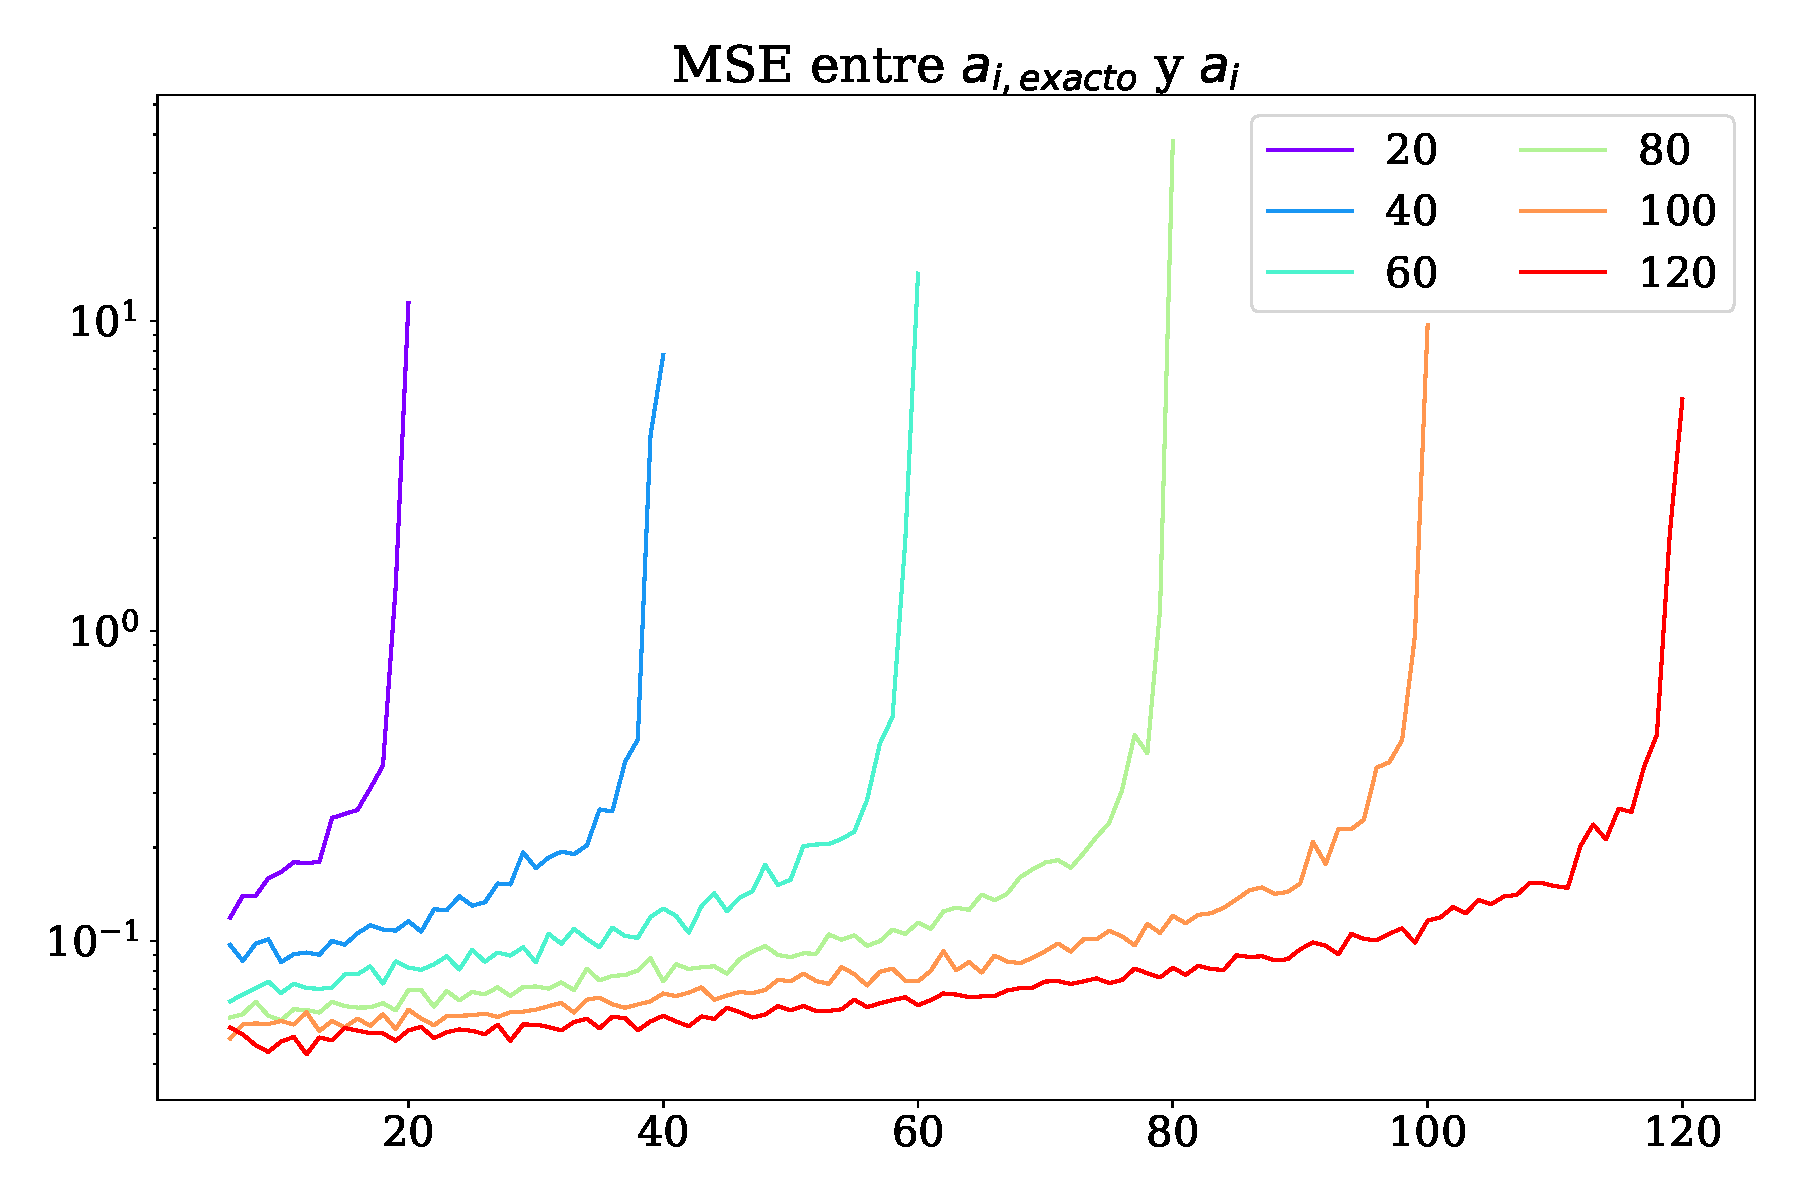
\includegraphics[width=0.49\textwidth]{ejer_1_mse_a_ejemplos.pdf}
        \caption{ejemplos}
        \label{fig:ejer1_a_ejemplos}
    \end{figure}

    \begin{figure}[H]
        \centering
        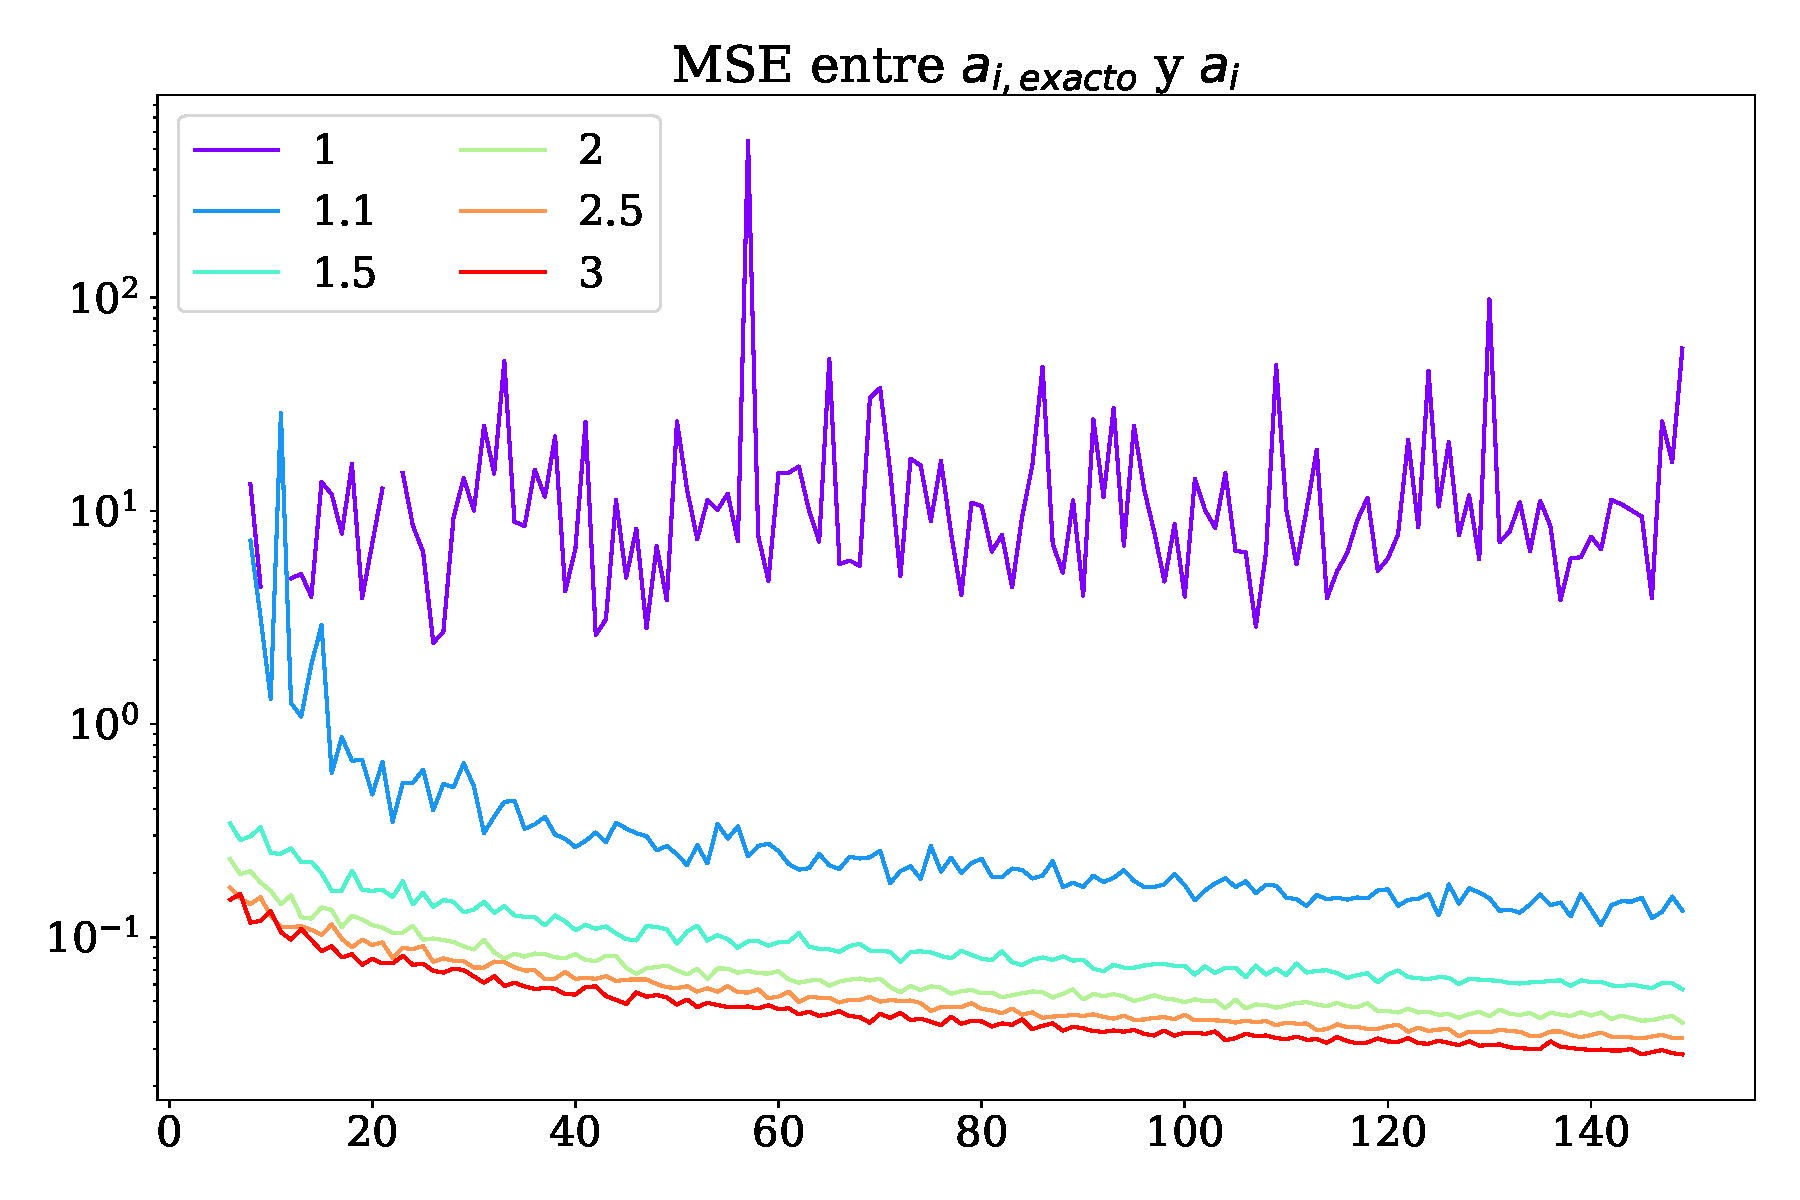
\includegraphics[width=0.5\textwidth]{ejer_1_mse_a_porcentaje.pdf}
        \caption{ejemplos}
        \label{fig:ejer1_a_porcentaje}
    \end{figure}

    \begin{figure}[H]
        \centering
        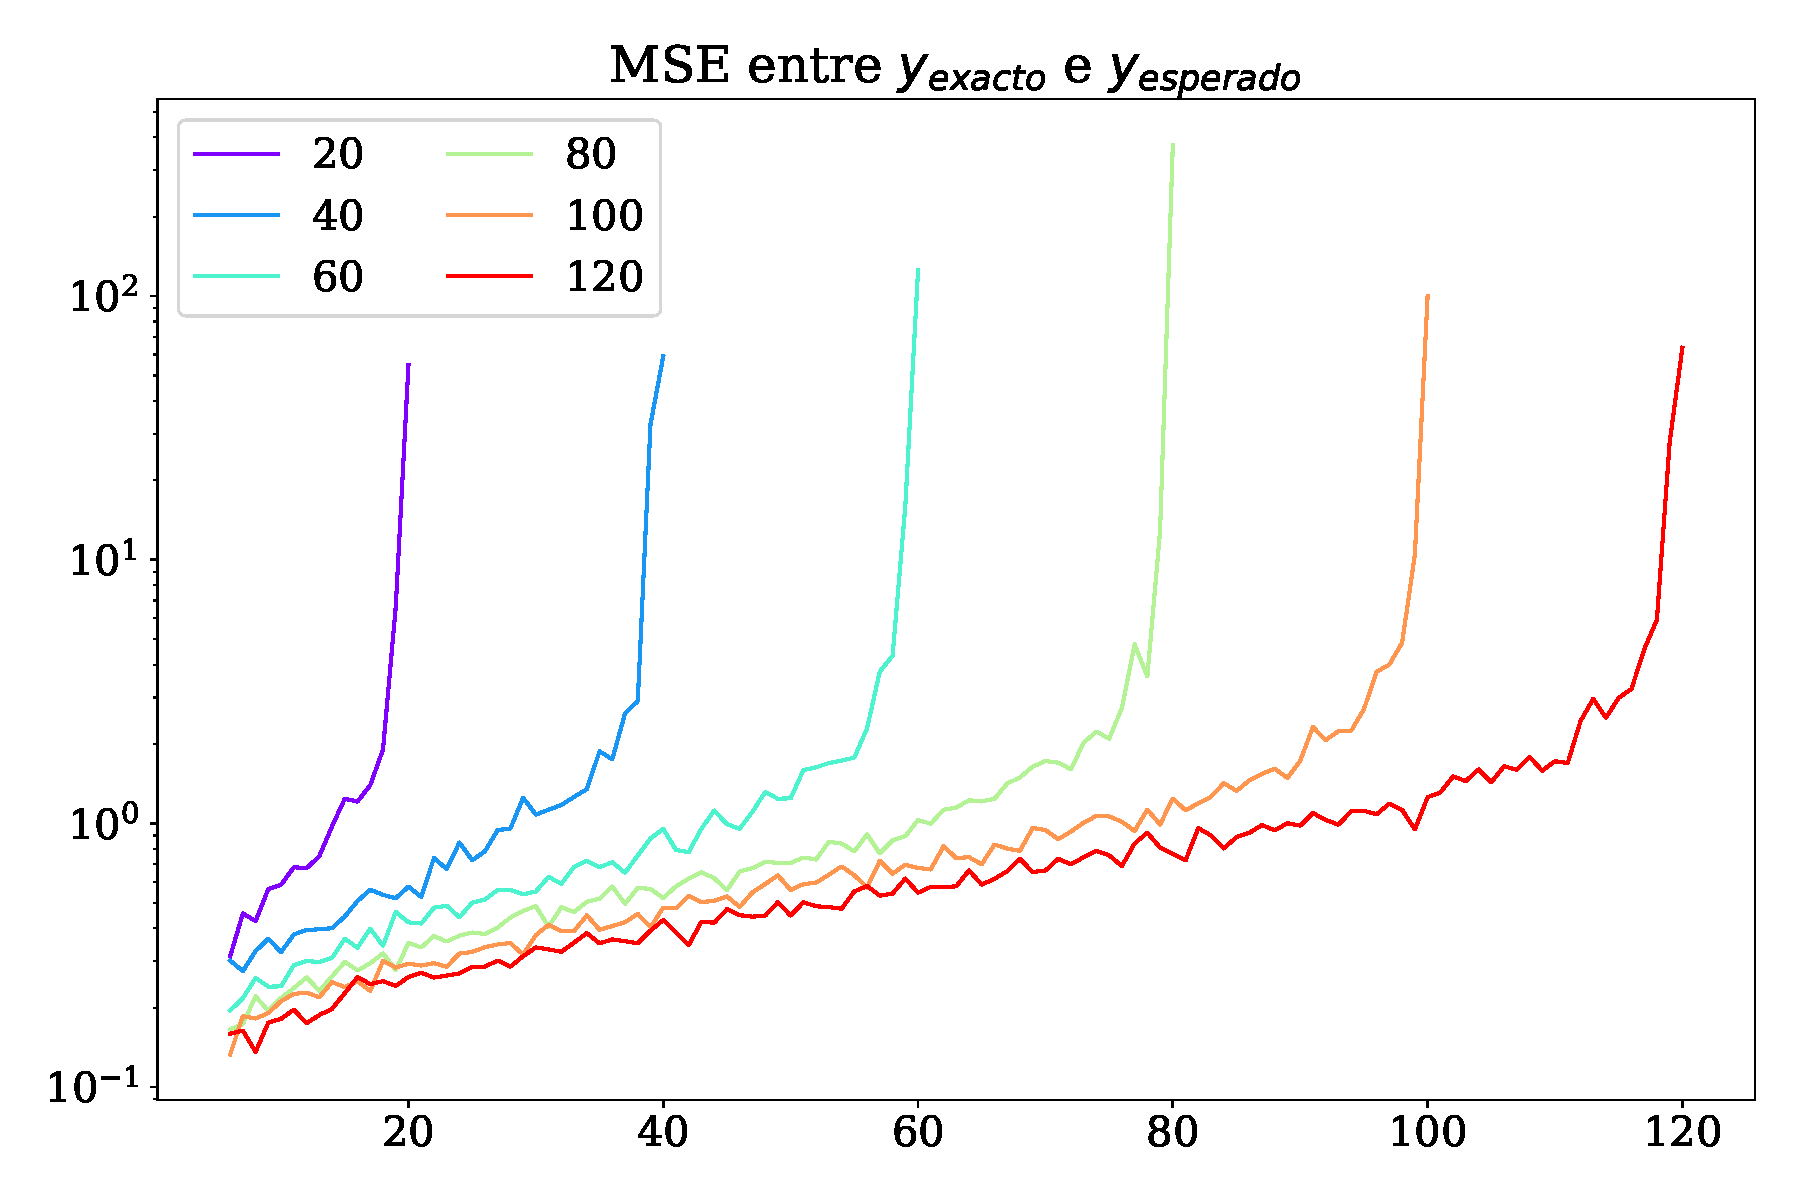
\includegraphics[width=0.5\textwidth]{ejer_1_mse_y_ejemplos.pdf}
        \caption{ejemplos}
        \label{fig:ejer1_y_ejemplos}
    \end{figure}

    \begin{figure}[H]
        \centering
        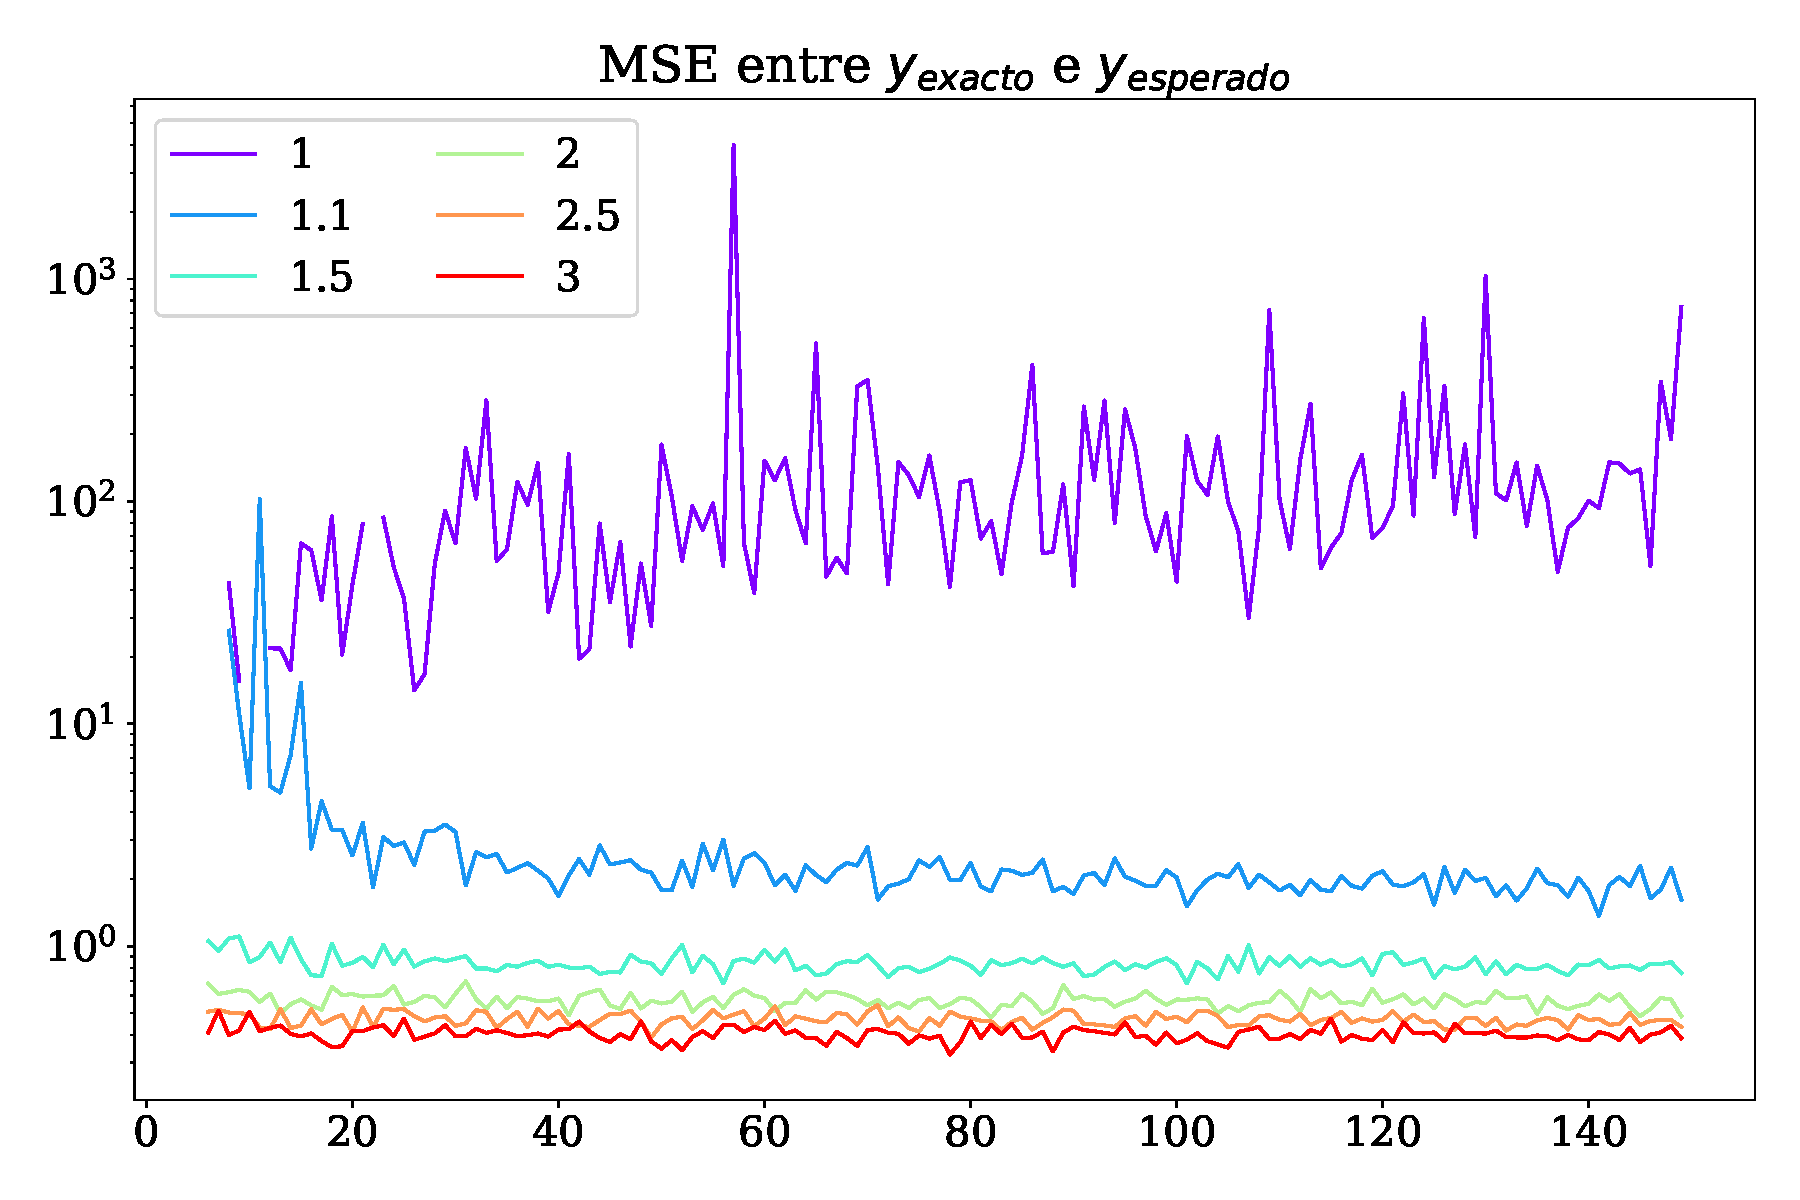
\includegraphics[width=0.5\textwidth]{ejer_1_mse_y_porcentaje.pdf}
        \caption{ejemplos}
        \label{fig:ejer1_y_porcentaje}
    \end{figure}


    \section*{Ejercicio 2}

    \begin{figure}[H]
        \centering
        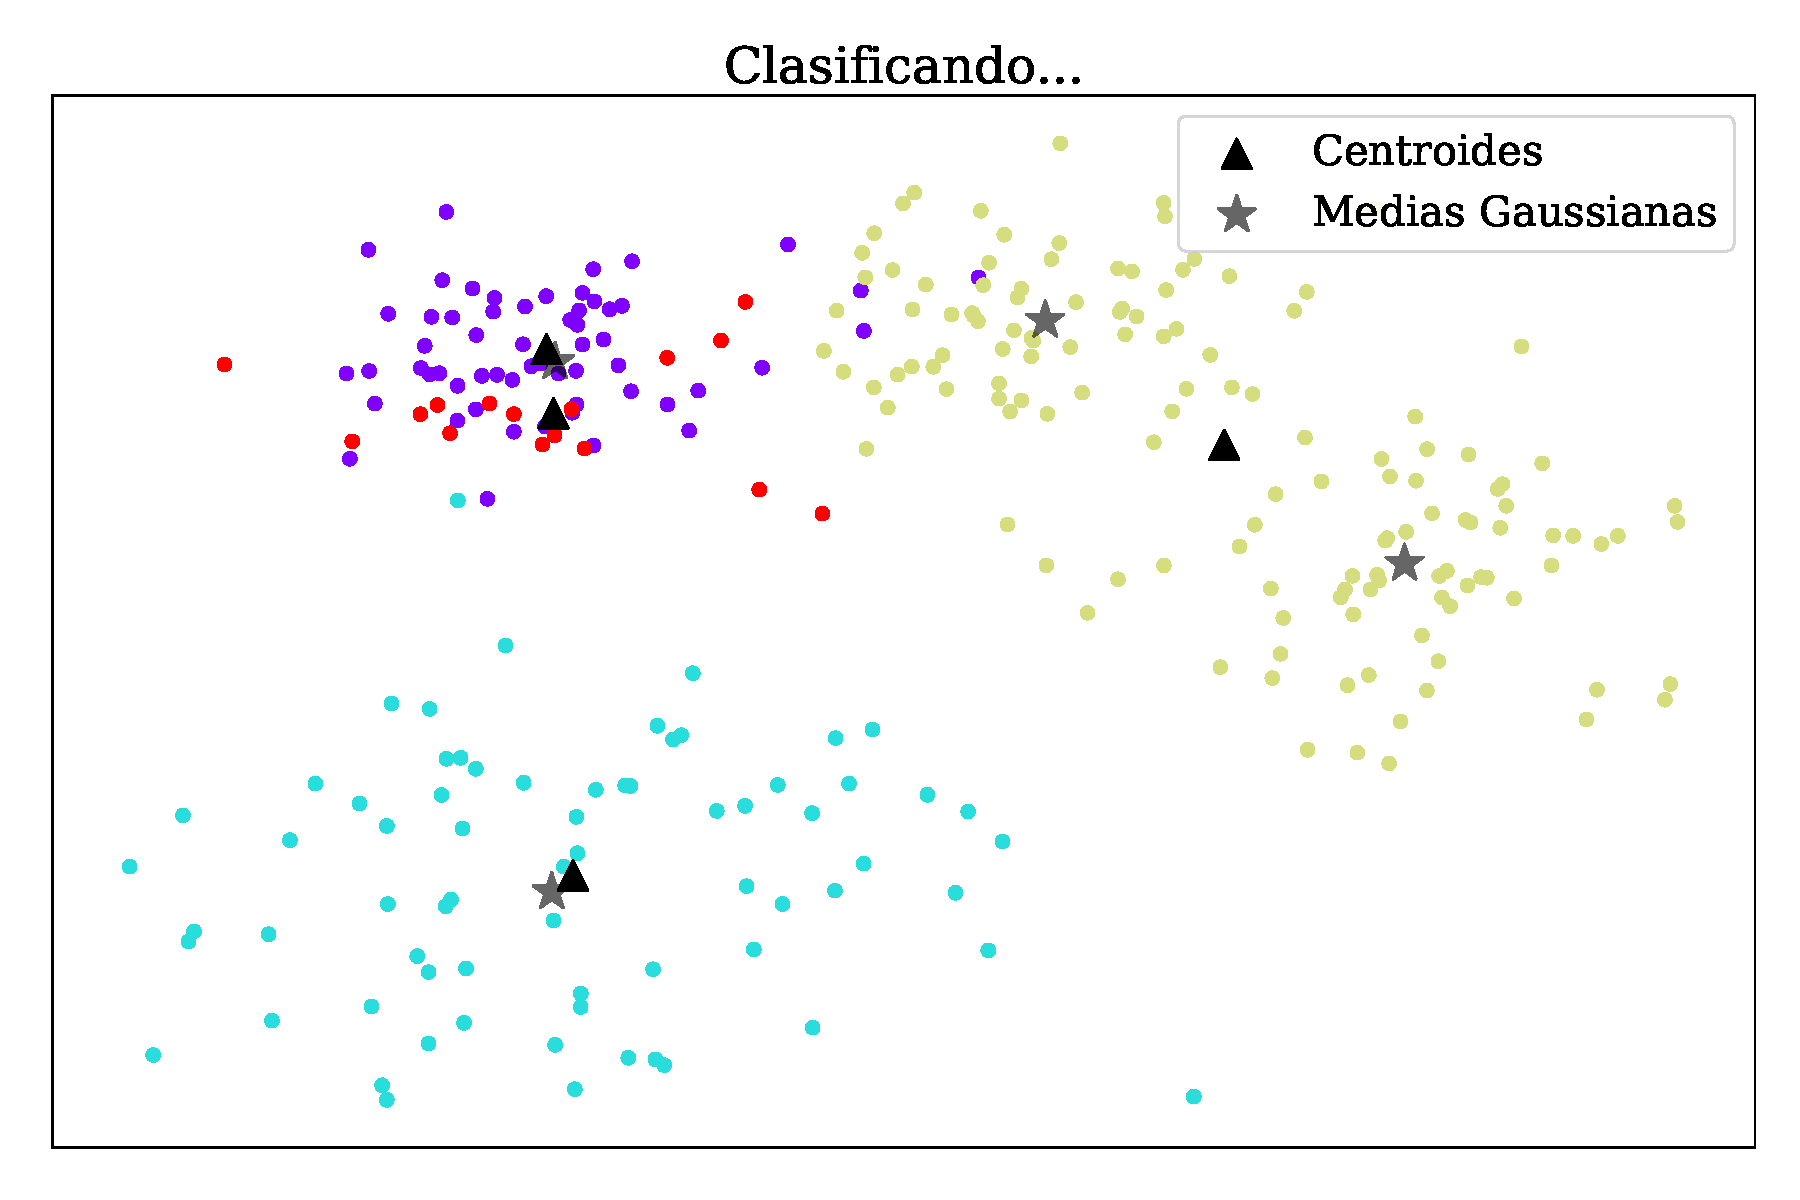
\includegraphics[width=0.5\textwidth]{ejer_2_clasificando_a_conv.pdf}
        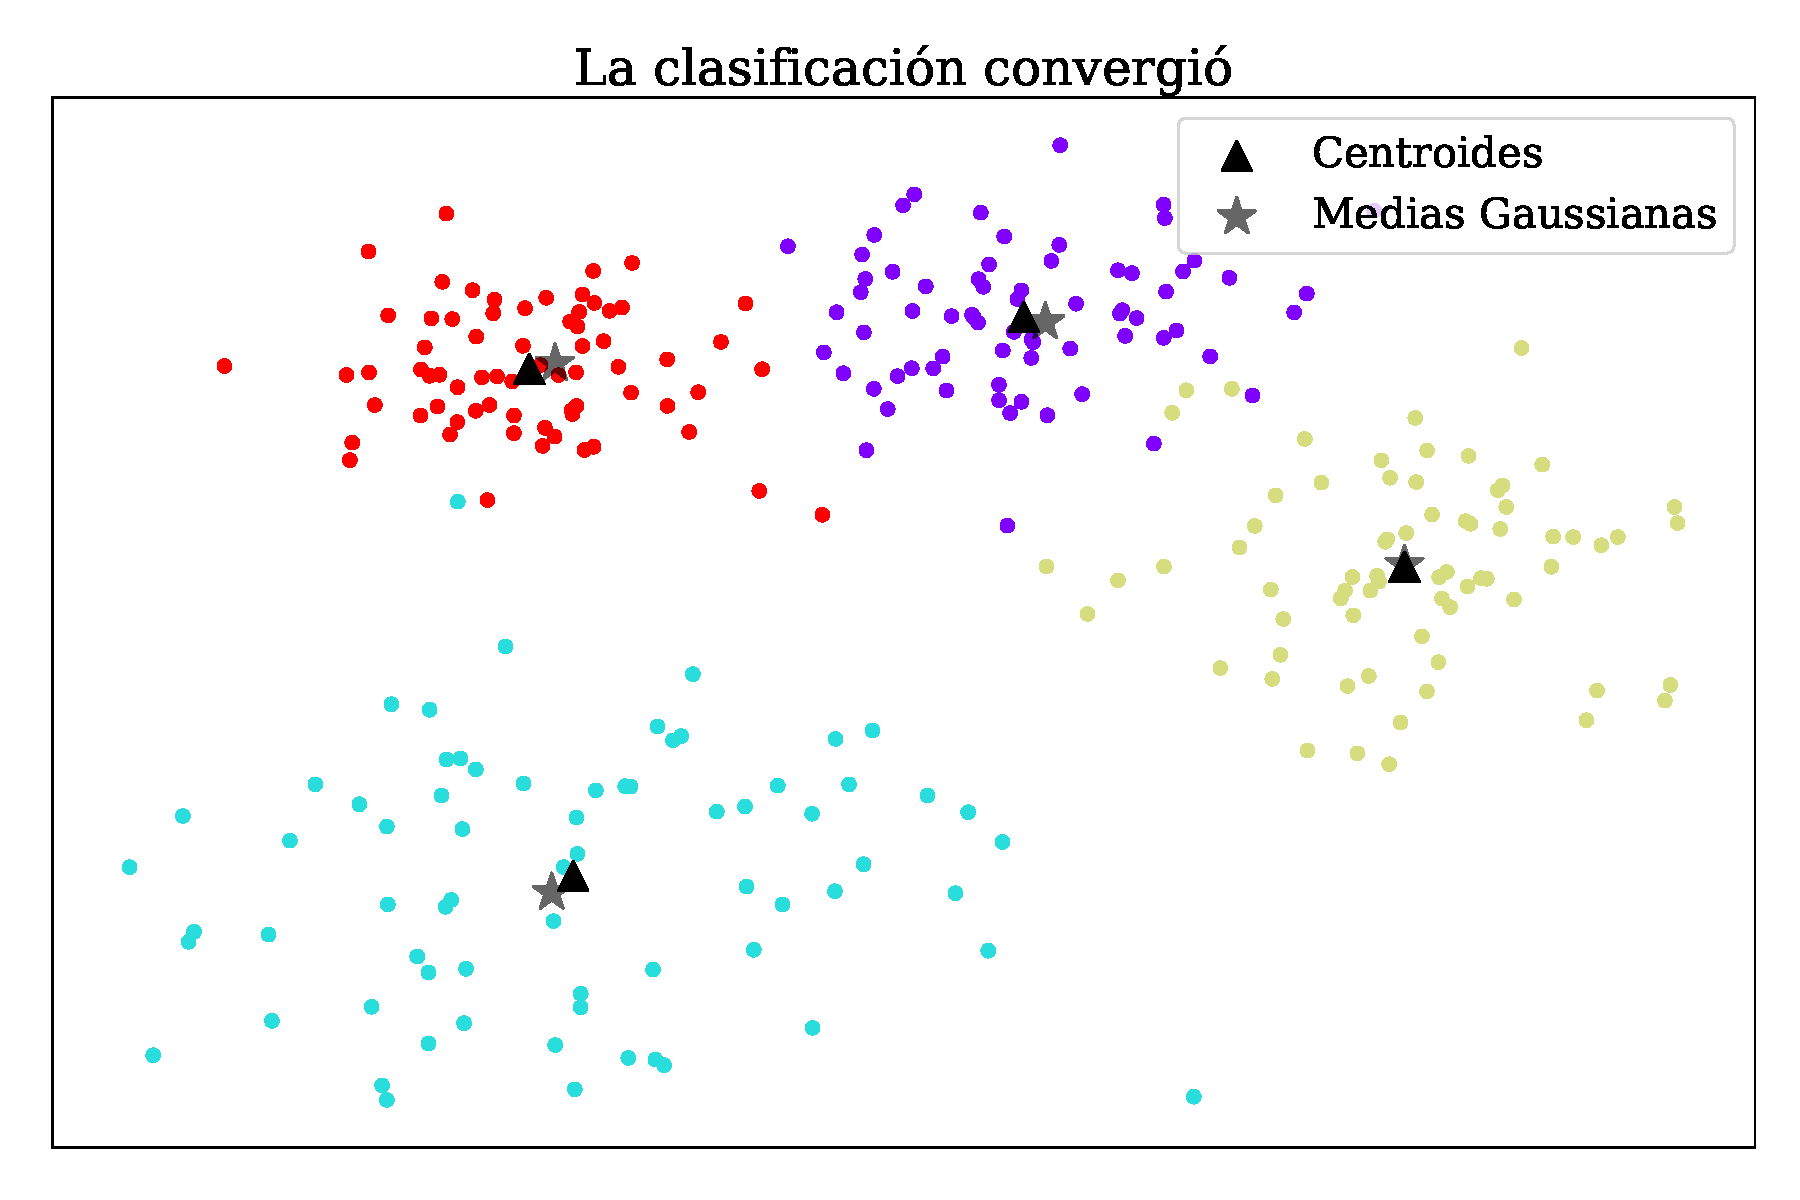
\includegraphics[width=0.5\textwidth]{ejer_2_si_converge.pdf}
        \caption{ejemplos}
        \label{fig:ejer2_converge}
    \end{figure}

    \begin{figure}[H]
        \centering
        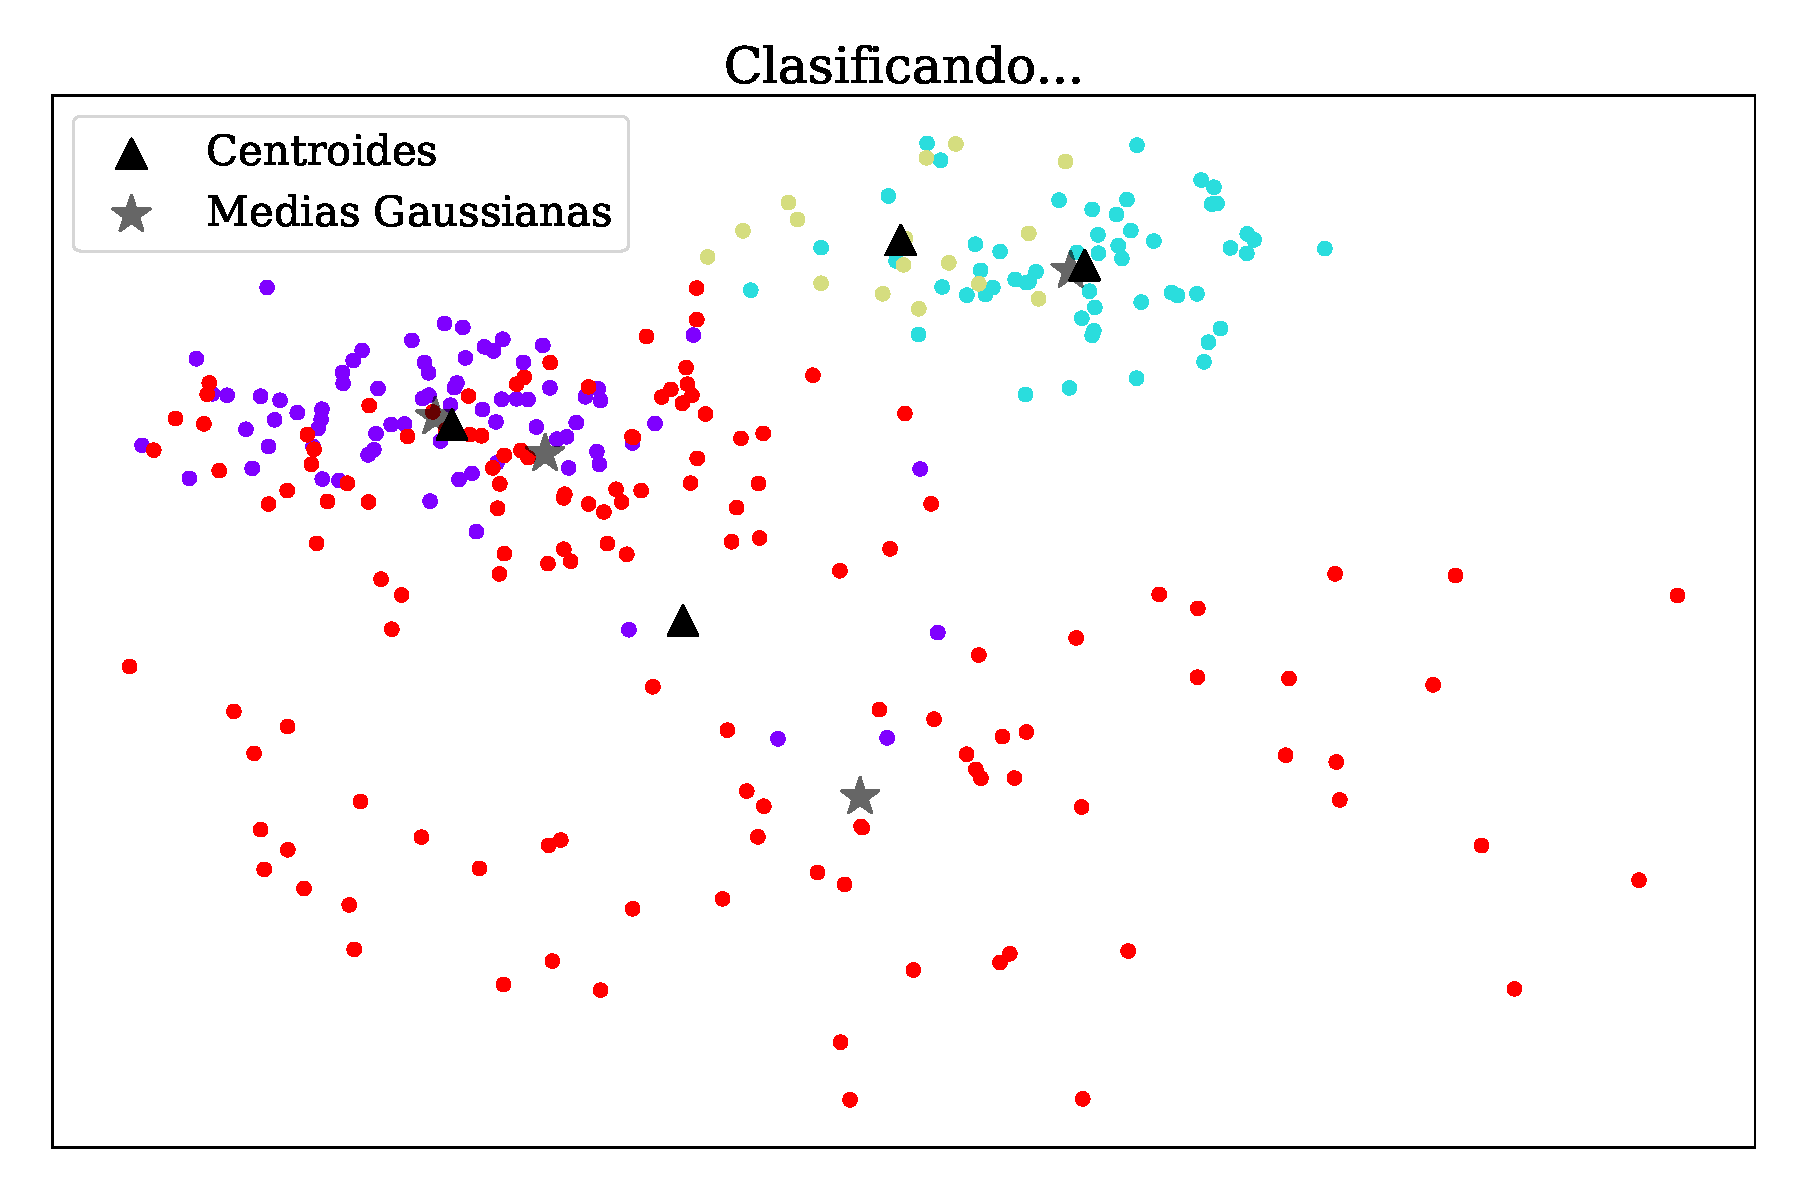
\includegraphics[width=0.5\textwidth]{ejer_2_clasificando.pdf}
        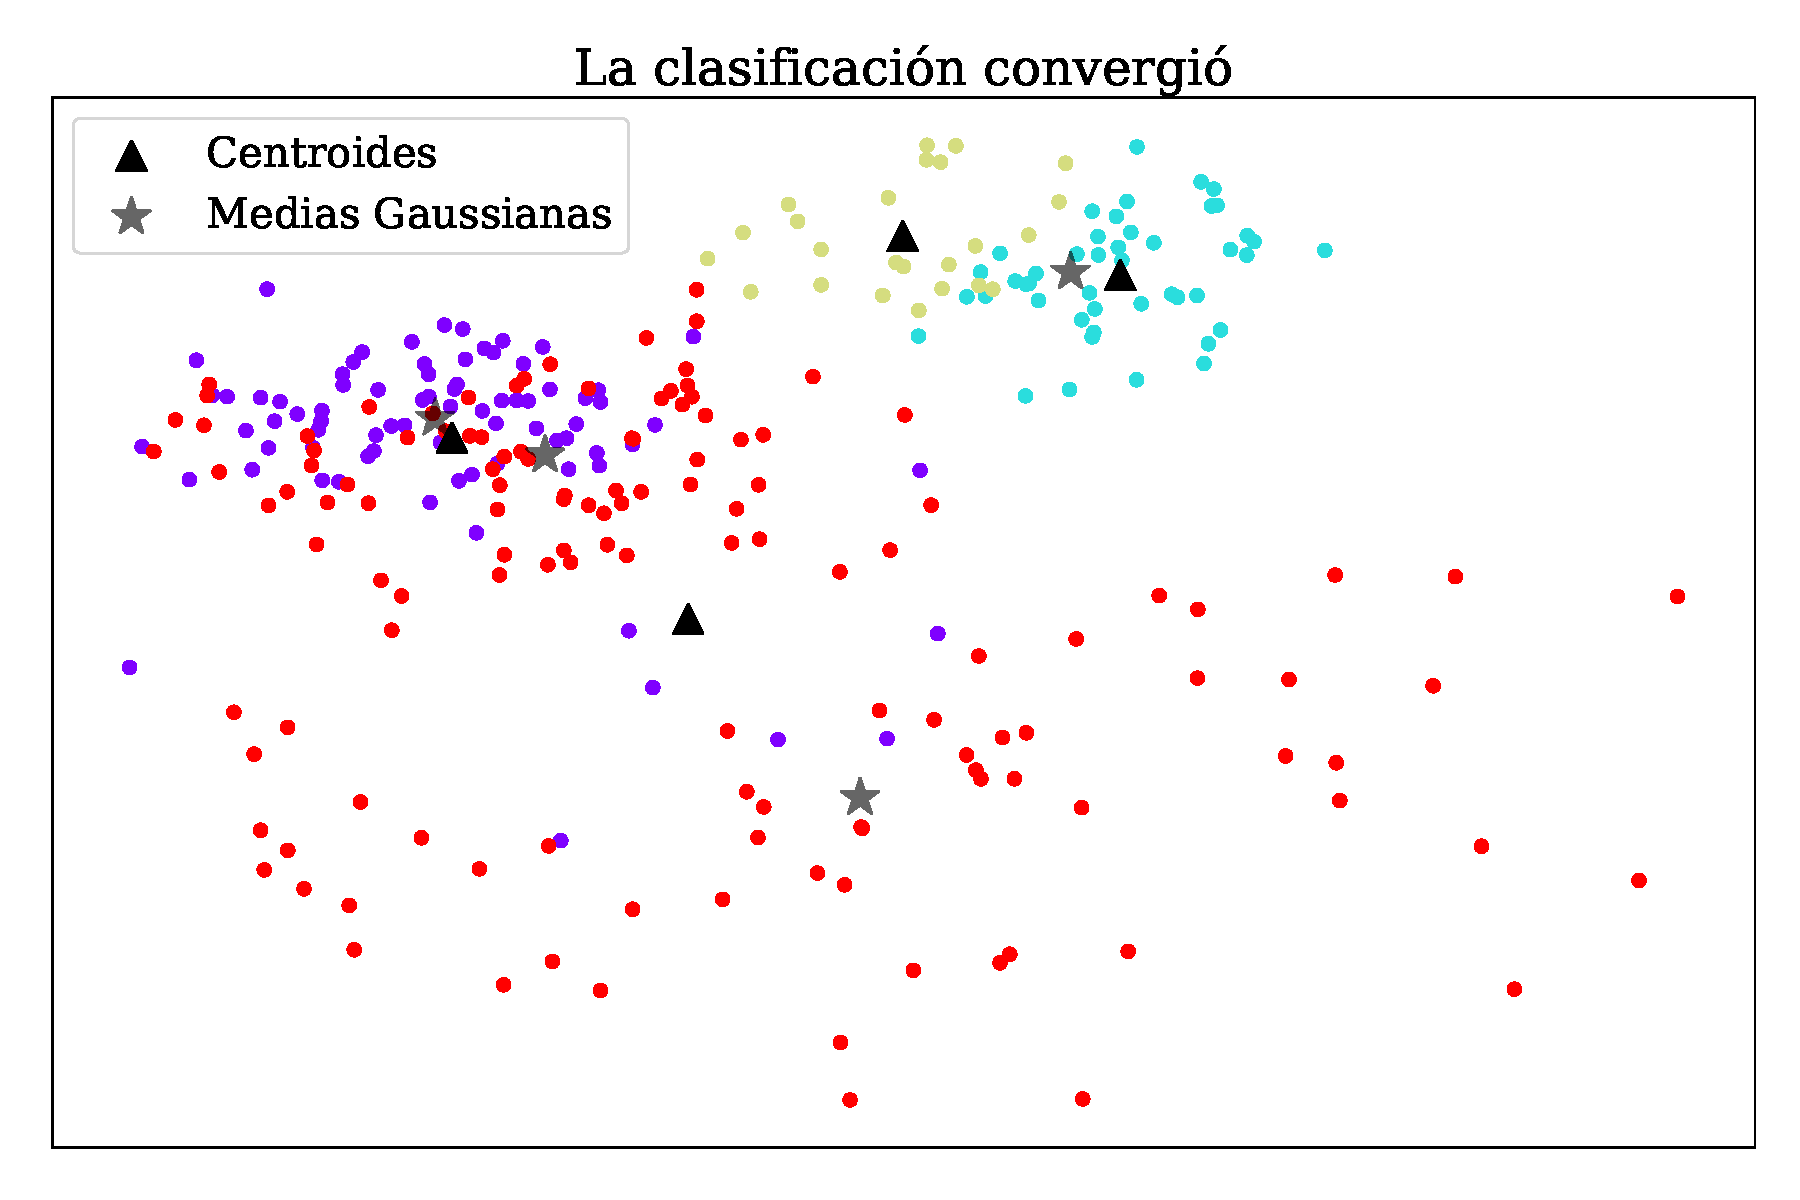
\includegraphics[width=0.5\textwidth]{ejer_2_no_converge.pdf}
        \caption{ejemplos}
        \label{fig:ejer2_no_converge}
    \end{figure}

    \section*{Ejercicio 4}



k=1
Dimensiones del set de entrenamiento  (375, 2)
375 ejemplos de entrenamiento
125 ejemplos para probar

36.0\% probando con 125 ejemplos

\begin{figure}[H]
    \centering
    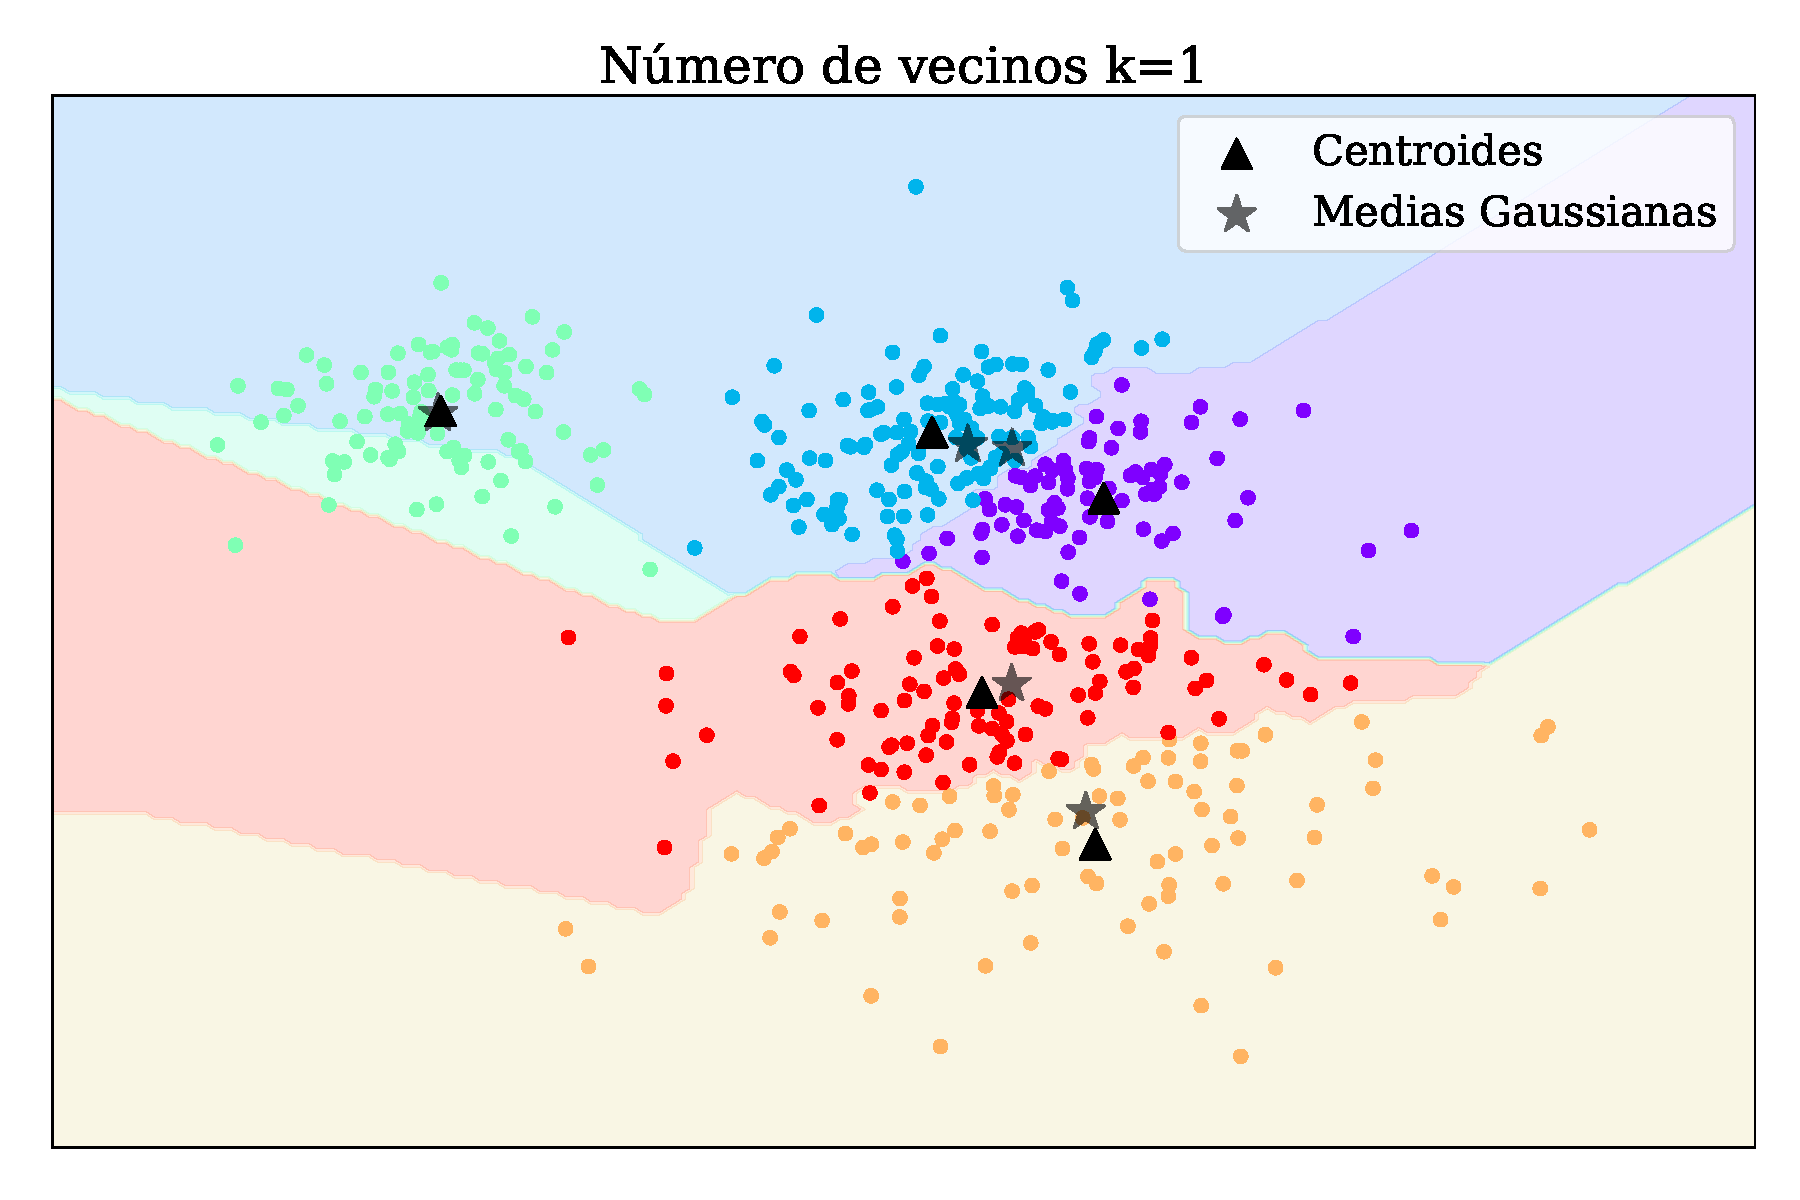
\includegraphics[width=0.5\textwidth]{ejer_4_K-1_no_coverge.pdf}
    \caption{K=1 malo}
    \label{fig:ejer4_k_1_malo}
\end{figure} 

k=1
Dimensiones del set de entrenamiento  (375, 2)
375 ejemplos de entrenamiento
125 ejemplos para probar

99.2\% probando con 125 ejemplos

\begin{figure}[H]
    \centering
    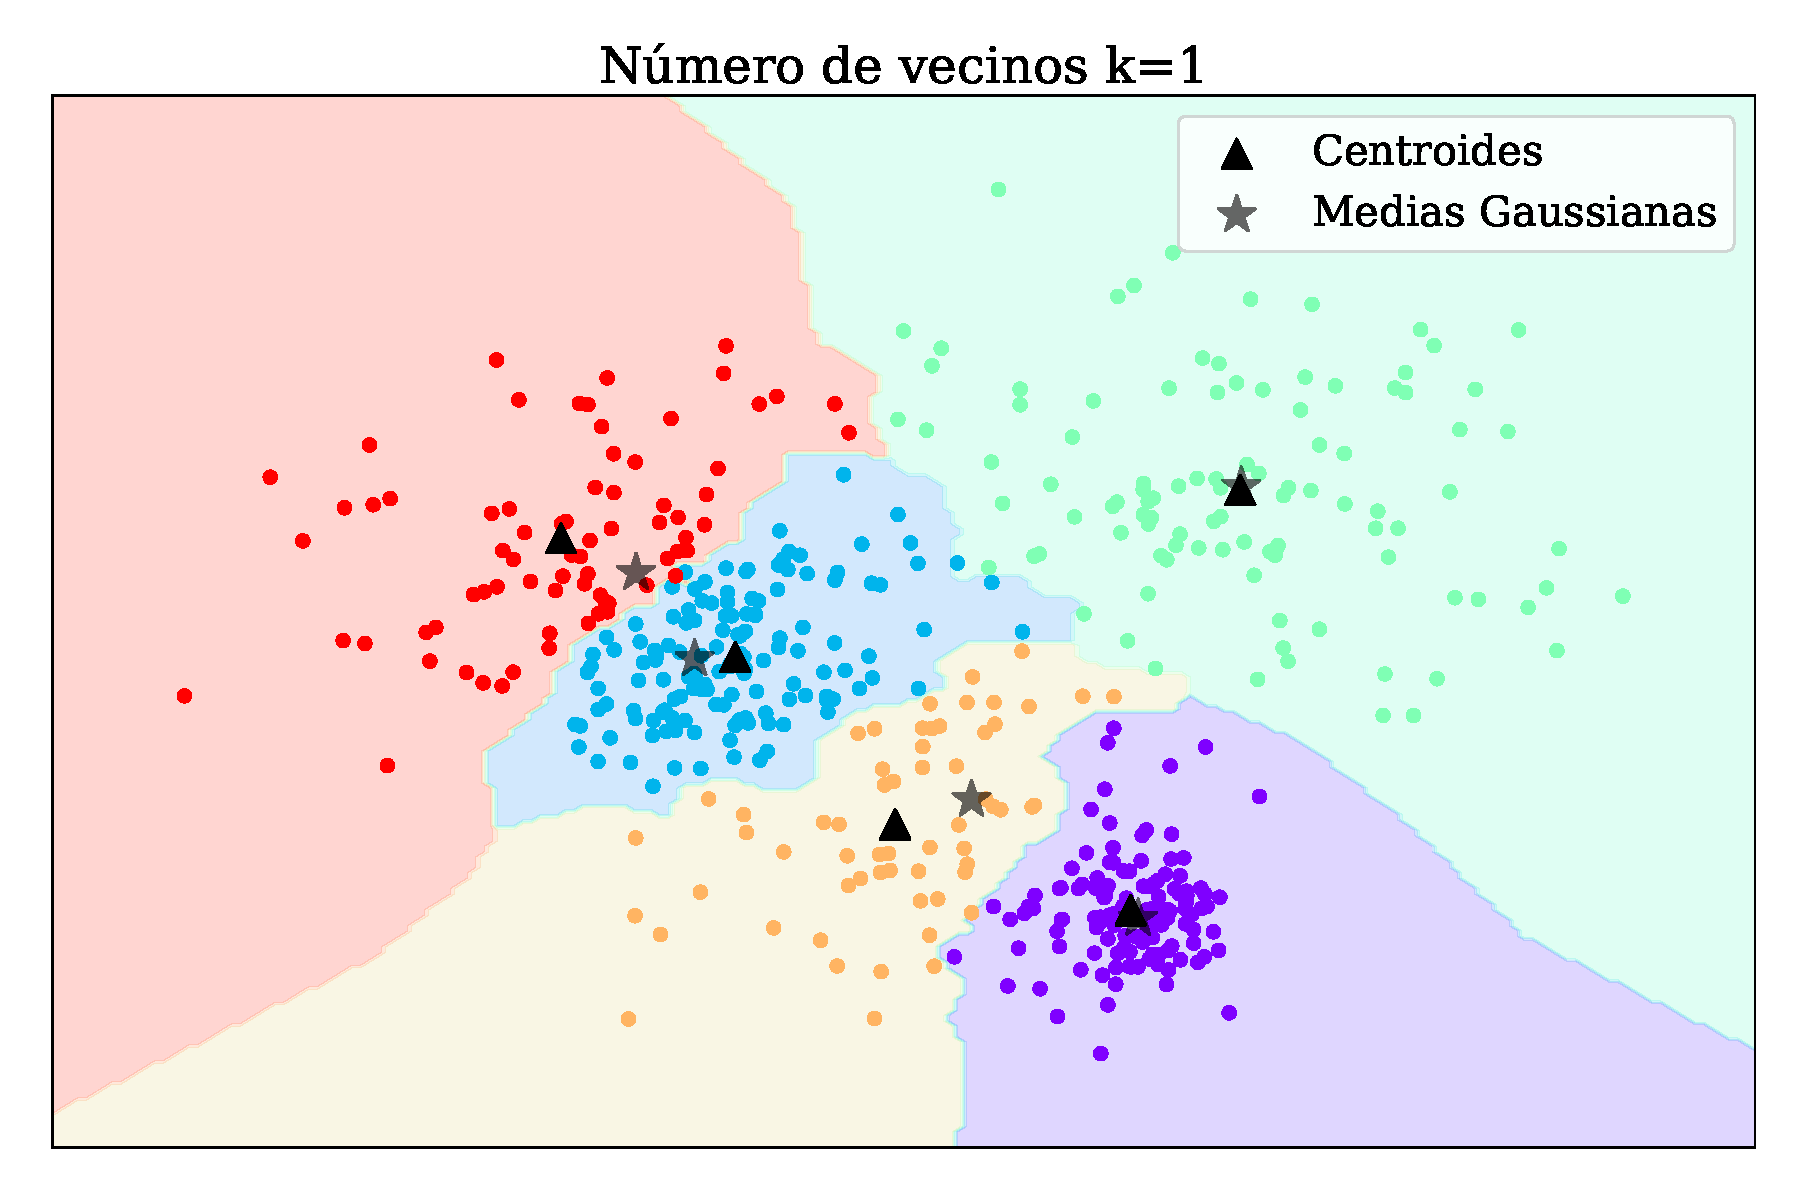
\includegraphics[width=0.5\textwidth]{ejer_4_K-1_si_converge.pdf}
    \caption{K=1 malo}
    \label{fig:ejer4_k_1}
\end{figure} 


k=3
Dimensiones del set de entrenamiento  (375, 2)
375 ejemplos de entrenamiento
125 ejemplos para probar

94.4\% probando con 125 ejemplos

\begin{figure}[H]
    \centering
    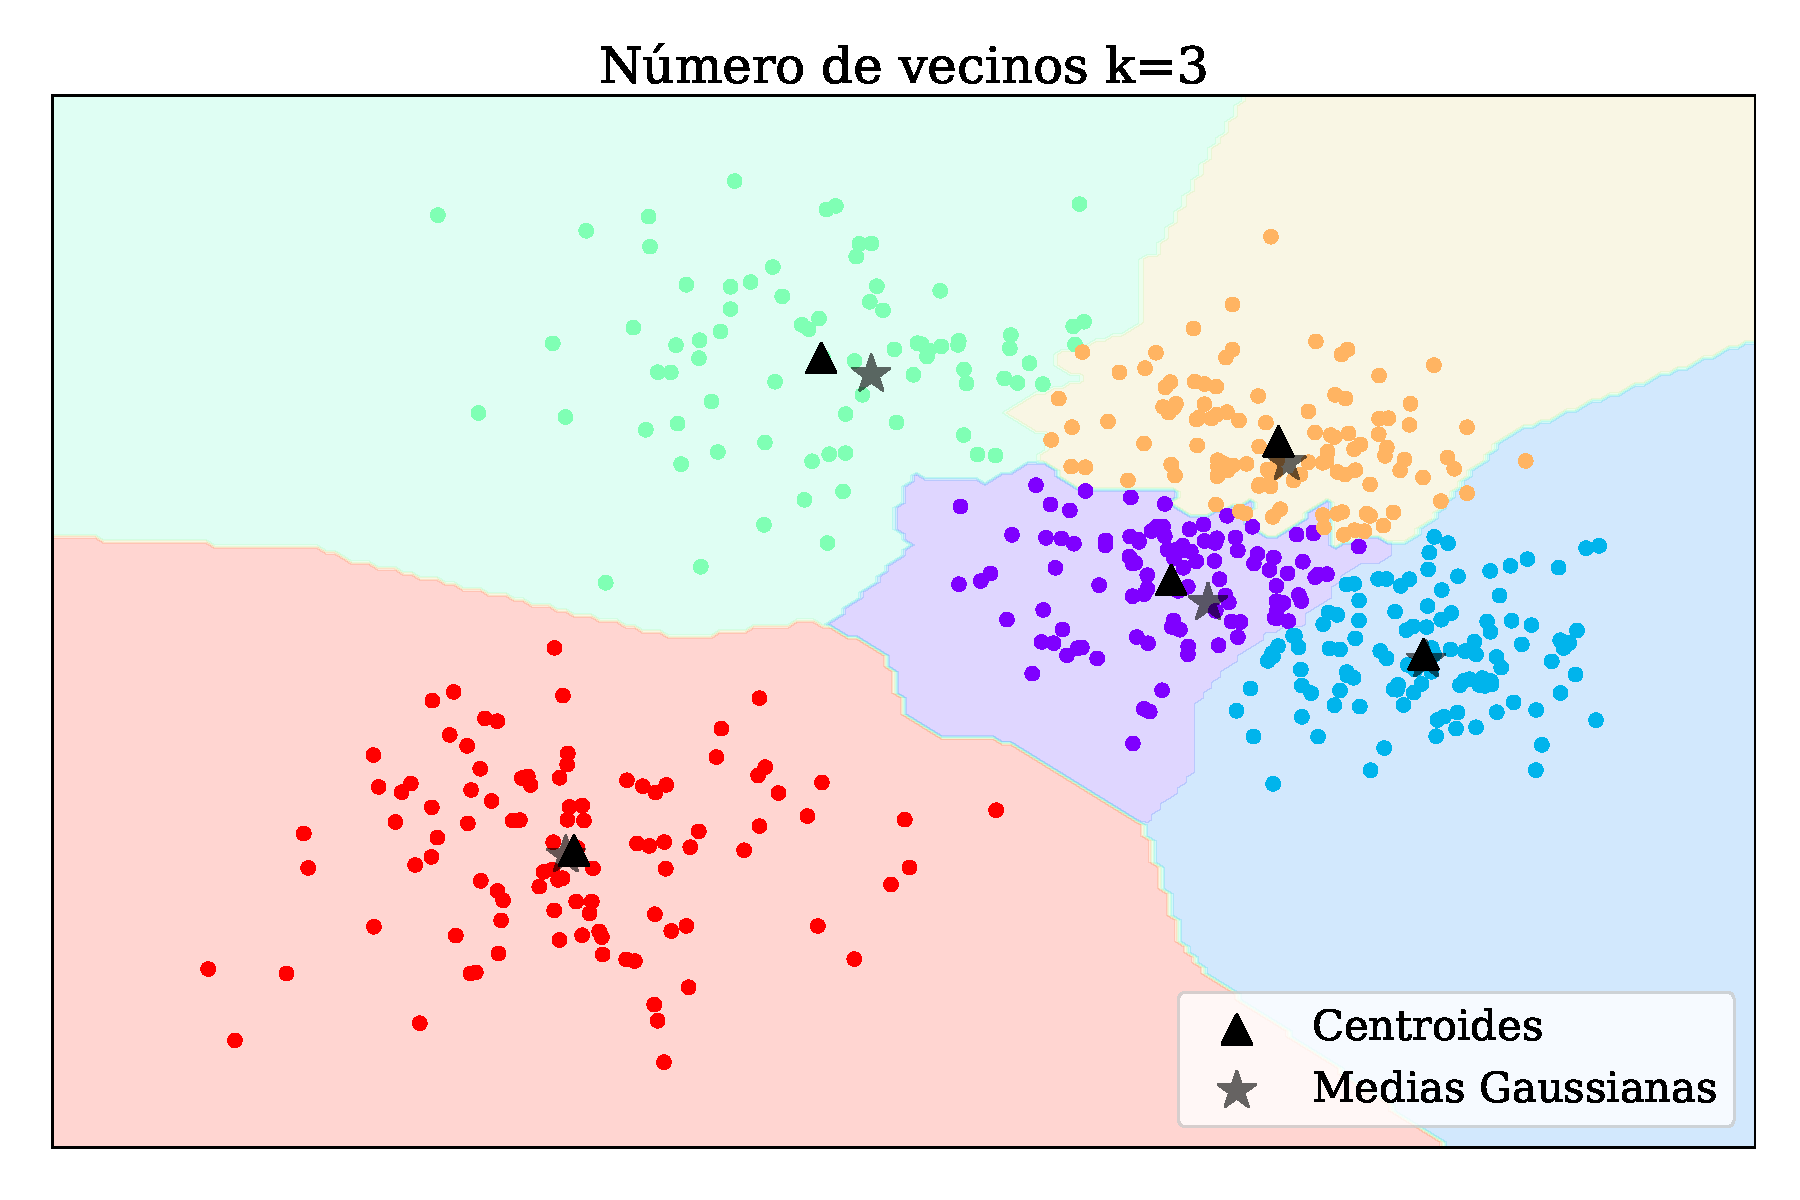
\includegraphics[width=0.5\textwidth]{ejer_4_K-3_si_converge.pdf}
    \caption{K=3 }
    \label{fig:ejer4_k_3}
\end{figure} 

k=7
Dimensiones del set de entrenamiento  (375, 2)
375 ejemplos de entrenamiento
125 ejemplos para probar

72.0\% probando con 125 ejemplos
\begin{figure}[H]
    \centering
    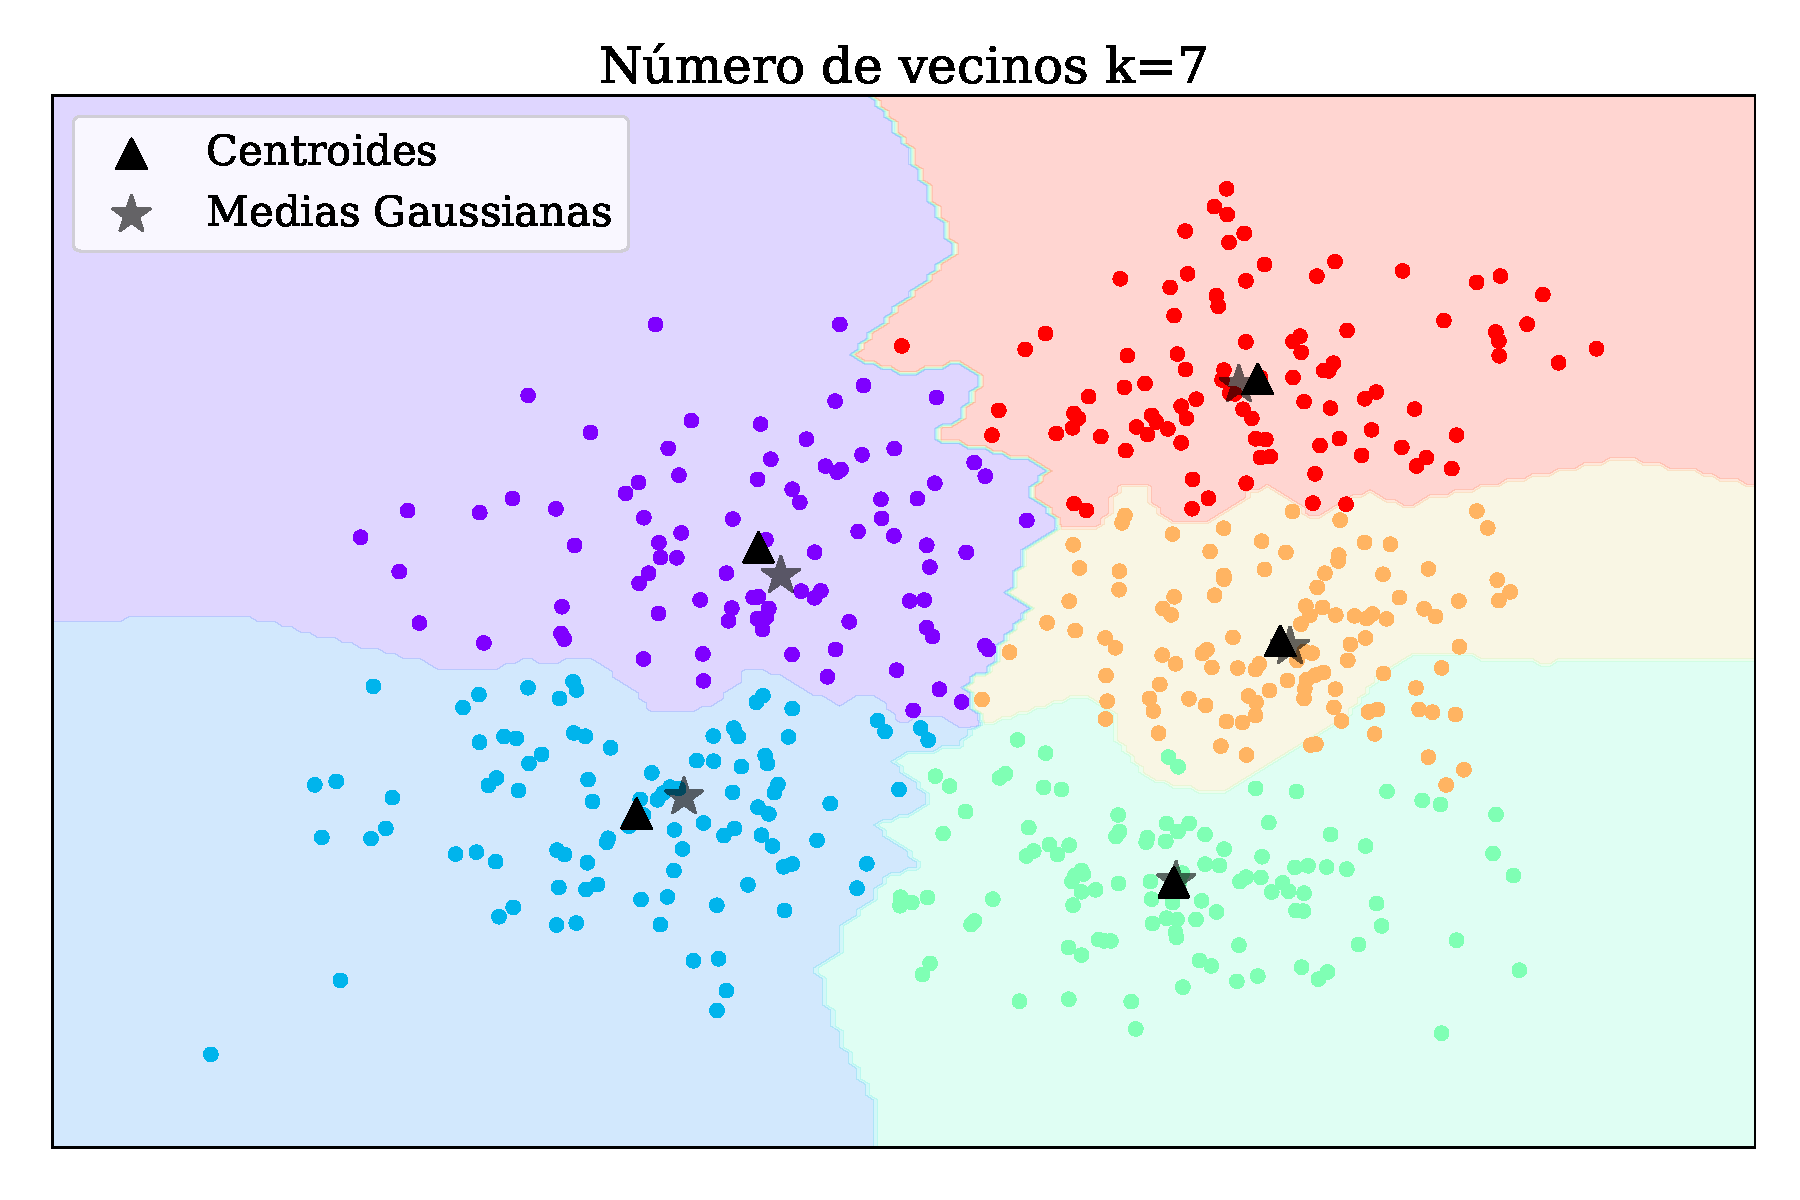
\includegraphics[width=0.5\textwidth]{ejer_4_K-7_si_converge.pdf}
    \caption{K=7 }
    \label{fig:ejer4_k_7}
\end{figure} 



\end{document}